\section{Introduction}

Models that can reason about the joint distribution of high-dimensional random variables are central to modern unsupervised machine learning. 
Explicit density evaluation is required in many statistical procedures,
while synthesis of novel examples can enable agents to imagine and plan in an environment prior to choosing a action.
In recent years, the variational autoencoder \citep[VAE,][]{Kingma:2014:vae, Rezende:2014:vae} and generative adversarial network \citep[GAN,][]{goodfellow:2014:gan} have received particular attention in the generative-modeling community, and both are capable of sampling with a single forward pass of a neural network. 
However, these models do not offer exact density evaluation, and can be difficult to train.
On the other hand, autoregressive density estimators \citep{uria2013rnade, germain2015made, oord2016pixelrnn, van2016pixelcnn, salimans2017pixelcnn++, van2016wavenet} can be trained by maximum likelihood,
but sampling requires a sequential loop over the output dimensions.

Flow-based models present an alternative approach to the above methods, and in some cases provide both exact density evaluation and sampling in a single neural-network pass.
A \emph{normalizing flow} models data $ \bfx $ as the output of an invertible, differentiable transformation $ \bff $ of noise $ \bfu $:
\begin{equation}
    \bfx = \bff\roundbr{\bfu}
    \quad\text{where}\quad
    \bfu\sim\pi\roundbr{\bfu}.
    \label{eq:flow_sampling}
\end{equation}
The probability density of $\bfx$ under the flow is obtained by a change of variables:
\begin{equation}
    p\roundbr{\bfx} = \pi\roundbr{\bff^{-1}\roundbr{\bfx}}\,\vertbr{\det\roundbr{\frac{\partial \bff^{-1}}{\partial\bfx}}}.
    \label{eq:flow-density}
\end{equation}
\begin{figure}
	\vspace{-1.0em}
    \centering
    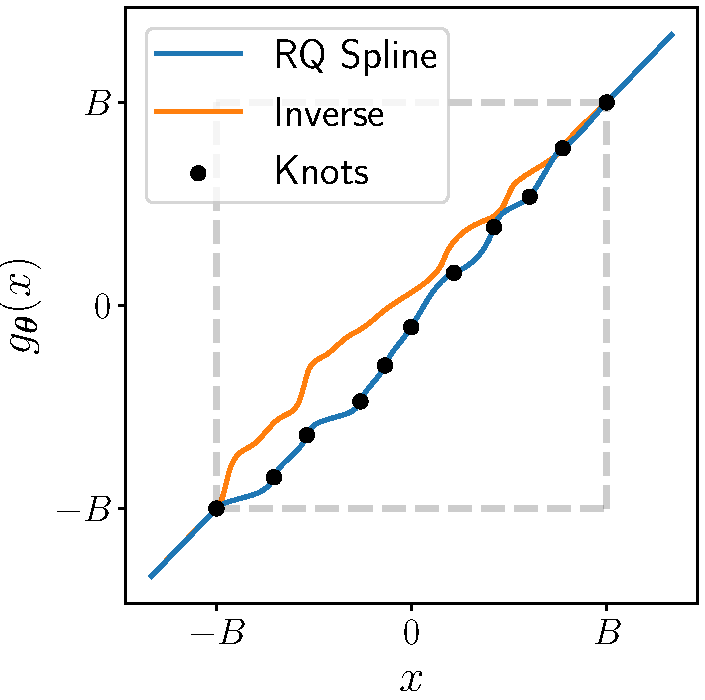
\includegraphics[width=0.3\textwidth]{figures/explanatory/rq-spline.pdf}
    \hspace{0.5cm}
    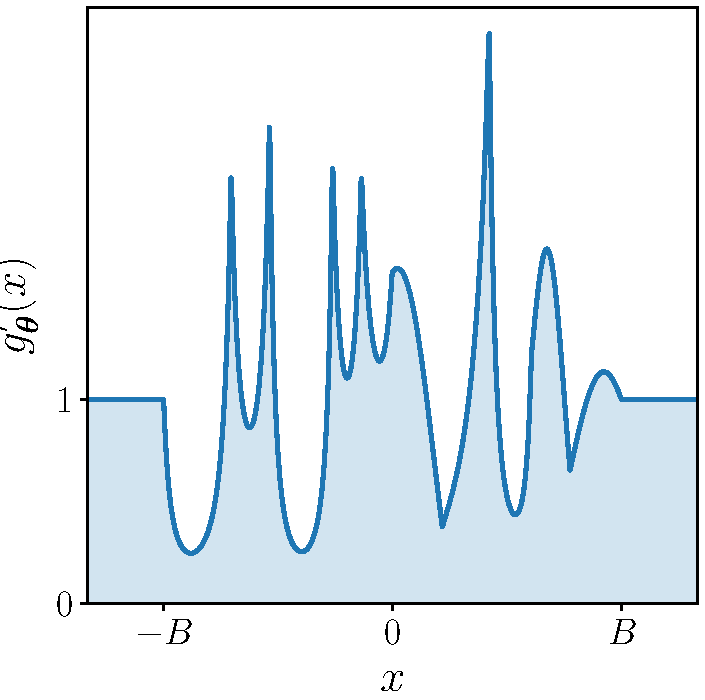
\includegraphics[width=0.3\textwidth]{figures/explanatory/rq-spline-derivative.pdf}
    \caption{Monotonic rational-quadratic transforms are drop-in replacements for additive or affine transformations in coupling or autoregressive layers, greatly enhancing their flexibility while retaining exact invertibility. \textbf{Left}: A random monotonic rational-quadratic transform with $ K = 10 $ bins and linear tails is parameterized by a series of $ K + 1 $ `knot' points in the plane, and the $ K - 1 $ derivatives at the internal knots. \textbf{Right}: Derivative of the transform on the left with respect to $x$. Monotonic rational-quadratic splines naturally induce multi-modality when used to transform random variables. }
    \label{fig:rq-spline}
    \vspace{-1.0em}
\end{figure}
Intuitively, the function $ \bff $ compresses and expands the density of the noise distribution $ \pi\roundbr{\bfu} $, and this change is quantified by the determinant of the Jacobian of the transformation. 
The noise distribution $\pi\roundbr{\bfu}$ is typically chosen to be simple, such as a standard normal, whereas the transformation $ \bff $ and its inverse $ \bff^{-1} $ are often implemented by composing a series of invertible neural-network modules. 
Given a dataset $\curlyD = \curlybr{\bfx^{(n)}}_{n=1}^{N}$, the flow is trained by maximizing the total log likelihood \smash{$\sum_n{\log p\roundbr{\bfx^{(n)}}}$} with respect to the parameters of the transformation $\bff$. In recent years, normalizing flows have received widespread attention in the machine-learning literature, seeing successful use in density estimation \citep{Dinh:2017:rnvp, Papamakarios:2017:maf}, variational inference \citep{Kingma:2016:iaf, Rezende:2015:flows, Louizos:2017:bnn, Berg:2018:sylvester}, image, audio and video generation \citep{Kingma:2018:glow, Kim:2018:FloWaveNet, Prenger:2018:WaveGlow, Kumar:2019:VideoFlow}, likelihood-free inference \citep{Papamakarios:2019:snl}, and learning maximum-entropy distributions \citep{Ganem:2017:max_entropy_flows}. 

A flow is defined by specifying the bijective function $\bff$ or its inverse $\bff^{-1}$, usually with a neural network. Depending on the flow's intended use cases, there are practical constraints in addition to formal invertibility:
\begin{itemize}[leftmargin=*, topsep=0pt, itemsep=0pt]
    \item To train a density estimator, we need to be able to evaluate the Jacobian determinant and the inverse function $\bff^{-1}$ quickly. We don't evaluate $\bff$, so the flow is usually defined by specifying $\bff^{-1}$.
    \item If we wish to draw samples using \cref{eq:flow_sampling}, we would like $\bff$ to be available analytically, rather than having to invert $\bff^{-1}$ with iterative or approximate methods.
    \item Ideally, we would like both $ \bff $ and $ \bff^{-1} $ to require only a single pass of a neural network to compute, so that both density evaluation and sampling can be performed quickly.
\end{itemize}
\emph{Autoregressive flows} such as inverse autoregressive flow \citep[IAF,][]{Kingma:2016:iaf} or masked autoregressive flow \citep[MAF,][]{Papamakarios:2017:maf} are $ D $ times slower to invert than to evaluate, where $ D $ is the dimensionality of $ \bfx $.
Subsequent work which enhances their flexibility has resulted in models which do not have an analytic inverse, and require numerical optimization to invert \citep{Huang:2018:naf}.
Flows based on \emph{coupling layers} \cite[NICE, RealNVP,][]{Dinh:2015:nice, Dinh:2017:rnvp} have an analytic one-pass inverse, but are often less flexible than their autoregressive counterparts. 

In this work, we propose a fully-differentiable module based on monotonic rational-quadratic splines which has an analytic inverse. 
The module acts as a drop-in replacement for the affine or additive transformations commonly found in coupling and autoregressive transforms. 
We demonstrate that this module significantly enhances the flexibility of both classes of flows, and in some cases brings the performance of coupling transforms on par with the best-known autoregressive flows. 
An illustration of our proposed transform is shown in \cref{fig:rq-spline}.
